% Automatic Metrics Table
\begin{table}[ht]
\centering
\caption{Automatic Evaluation Metrics}
\label{tab:automatic-metrics}
\begin{tabular}{lcc}
\toprule
\textbf{Metric} & \textbf{Baseline} & \textbf{Controlled} \\
\midrule
BLEU & 9.57 & 9.16 \\
ROUGE-1 & 0.365 & 0.349 \\
ROUGE-2 & 0.156 & 0.150 \\
ROUGE-L & 0.318 & 0.303 \\
\bottomrule
\end{tabular}
\end{table}

% QA Answerability Table
\begin{table}[ht]
\centering
\caption{QA Answerability Metrics}
\label{tab:qa-metrics}
\begin{tabular}{lcc}
\toprule
\textbf{Metric} & \textbf{Baseline} & \textbf{Controlled} \\
\midrule
Exact Match (EM) & 0.145 & 0.110 \\
F1 Score & 0.233 & 0.211 \\
\bottomrule
\end{tabular}
\end{table}

% Comparison Figure
\begin{figure}[ht]
\centering
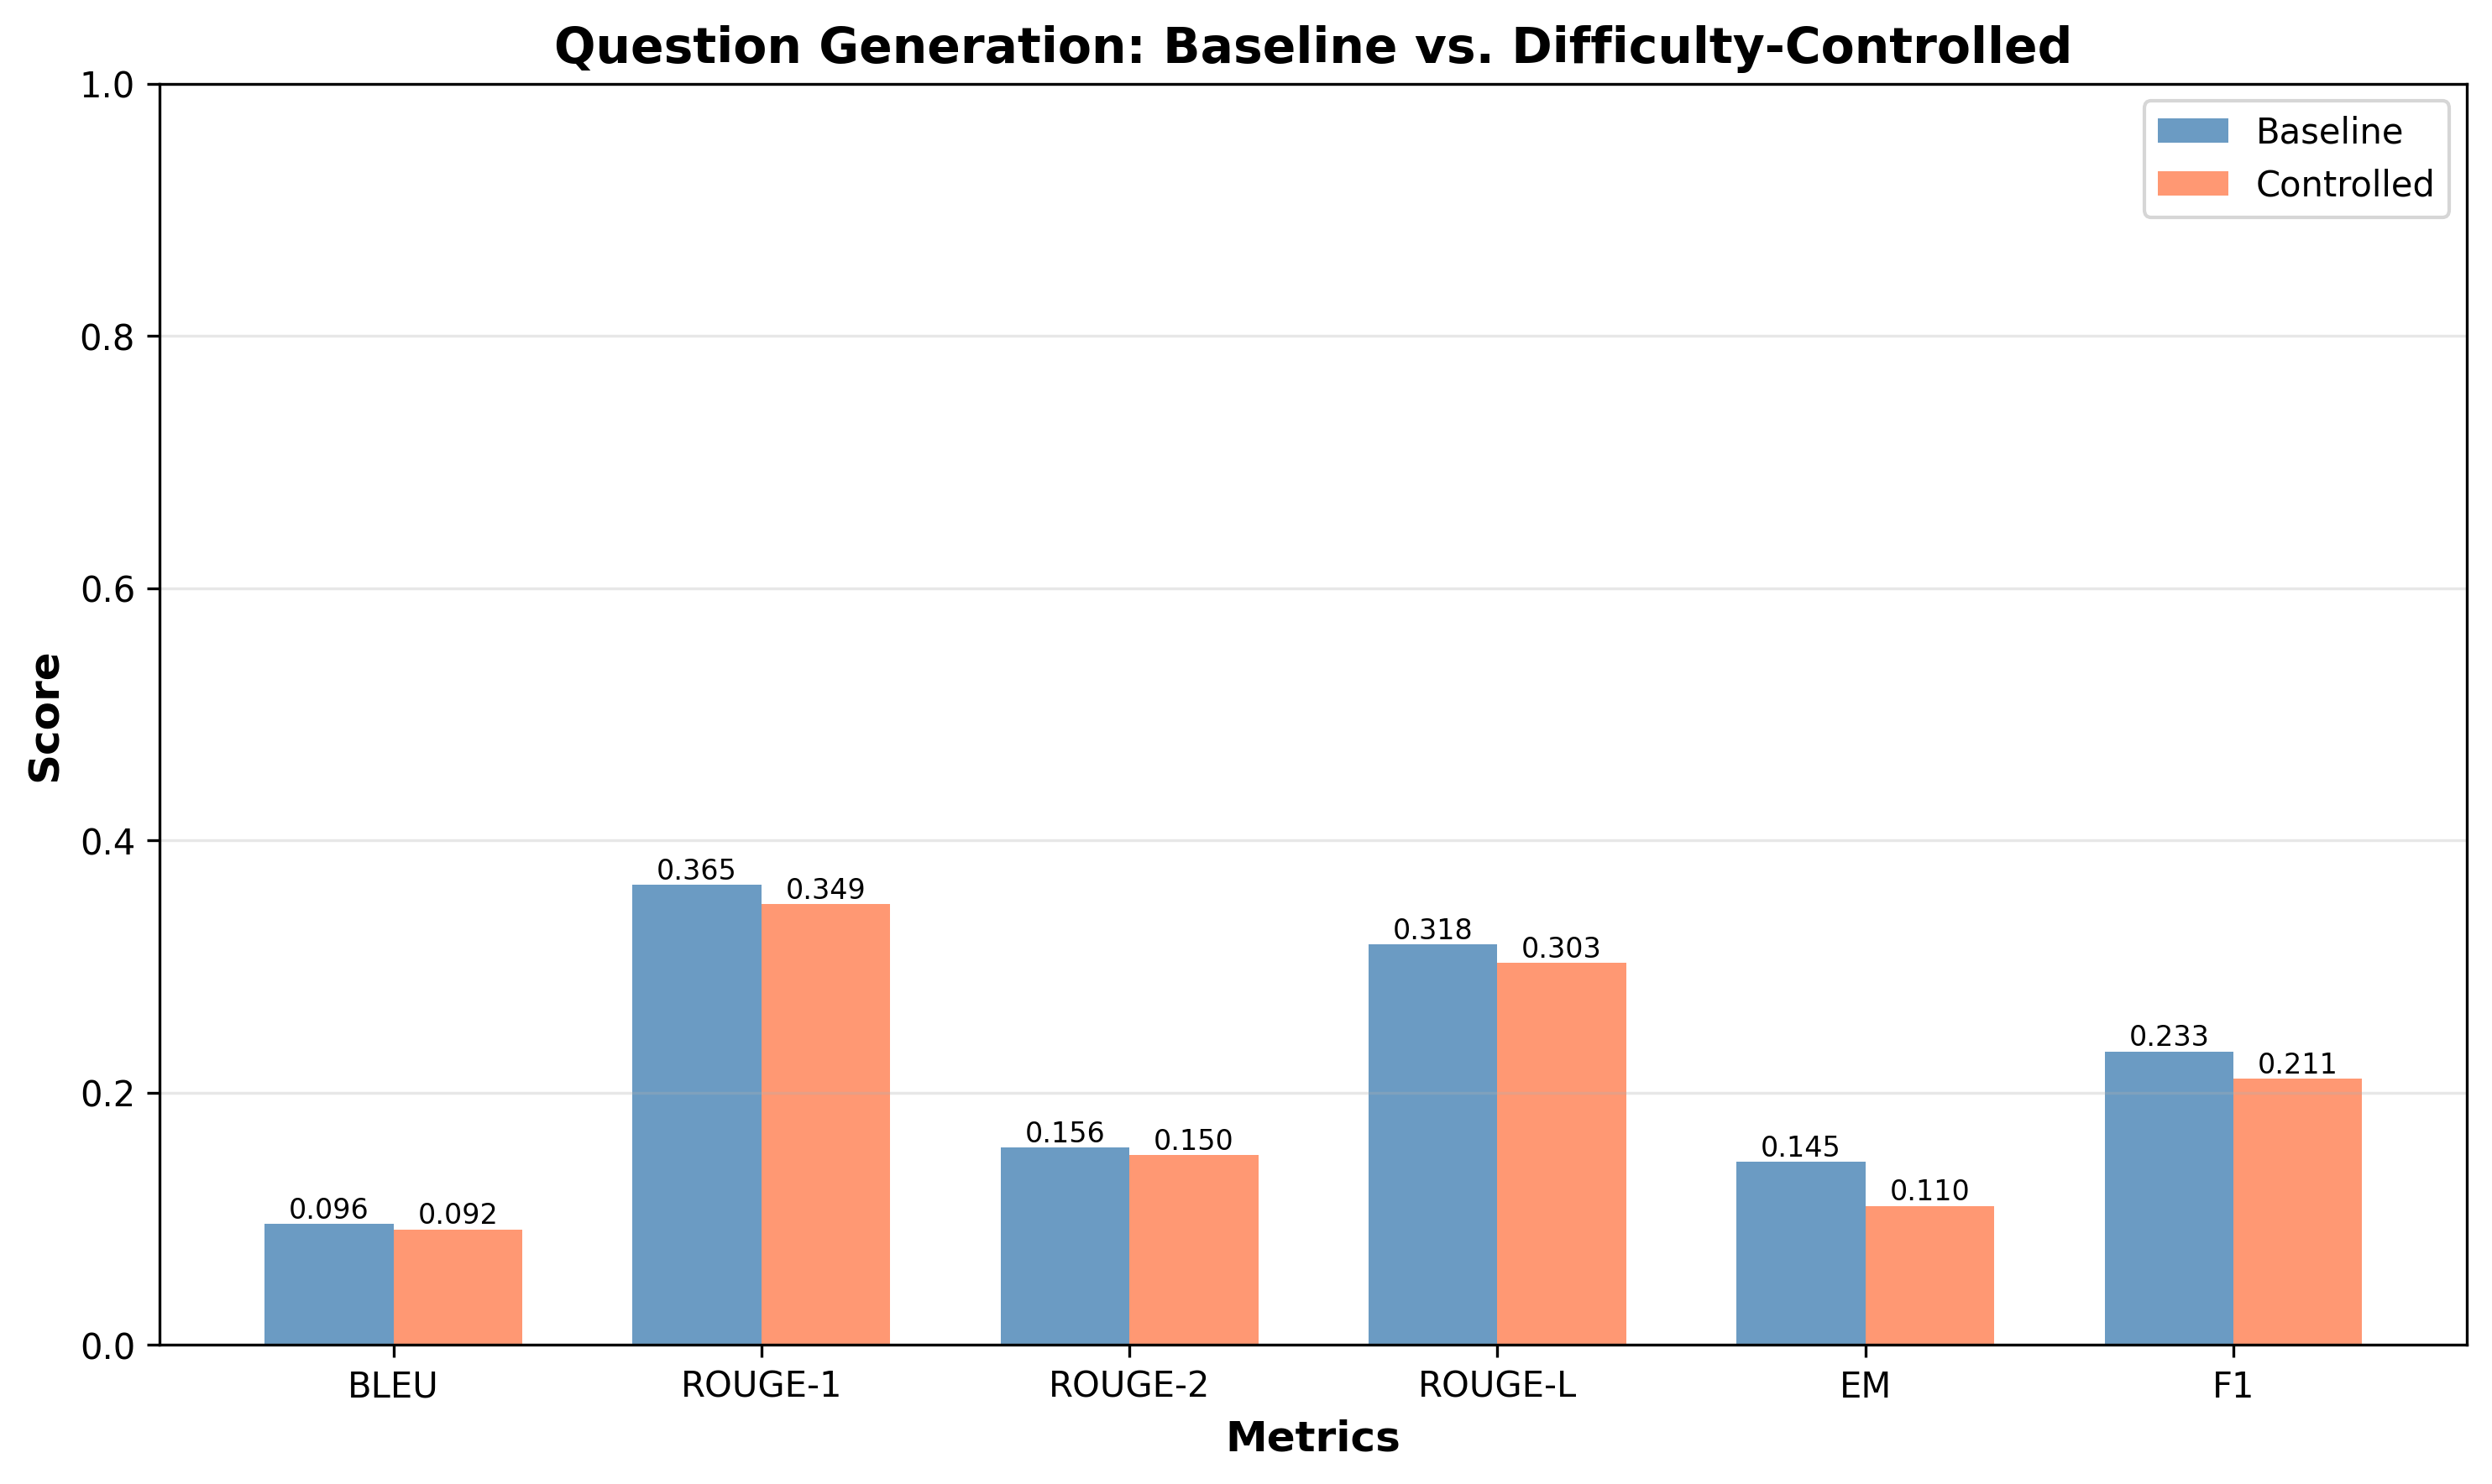
\includegraphics[width=0.8\textwidth]{../reports/figures/comparison_squad.png}
\caption{Comparison of baseline and difficulty-controlled question generation systems.}
\label{fig:comparison}
\end{figure}
